\chapter{Boring stuff}
\section{Version History}
\begin{description}
\item[v 0.1 2016:] This project is begun in a trio of physical exercise books as \textit{The Little Book of Physics Formulae}, \textit{The Little Book of Mathematics Formulae}, and \textit{The Little Book of Astronomy Formulae}
\item[v 0.6 2016:] The process of transferring the formulae from paper to LaTeX is initiated, but abandoned (or drifted away from).
\item[v 0.7 2018-03-20:] The project is resurrected (probably because the author started MRes), uploaded to Overleaf, and cleaned up.
\item[v 0.8 2018-07-12:] Remaining formulae imported from the original books.
\item[v 0.9 2018-07-26:] Further formulae imported from undergrad formula sheets.
\item[v 1.0 2018-07-28:] First public release, with some additions from 0.9.
\item[v 1.0.1 2018-07-31:] Minor corrections, added "dynamical timescale" (2.2.2) and some more formulae to the Statistics chapter (it was looking a little bare).
\item[v 1.1 xxxx:] Font change; added Planck units and some other miscellaneous units to Units of Measurement; fine structure constant to Physical Constants (why wasn't it already there?); stellar luminosity; formulae for Green's functions and other differential equation techniques; minor corrections; Gaussian distributions to Statistics section.
\end{description}

\section{Licensing}

\doclicenseThis
    
(Basically, as long as you credit me and share under a similar license, feel free to use this however you want)

\section{Contact}
    	
Visit www.webofworlds.net for science fiction, science fact, geeky opinions, and maybe some Python code. \\ 
Suggestions or corrections are welcome at webofworlds@gmail.com

\section{Credits}

\begin{description}
\item [Formula Sheets: Audrey Markowskei, ] 
\item [Unit Circle:] By Jim.belk [CC BY-SA 3.0 (https://creativecommons.org/licenses/by-sa/3.0) or GFDL (\url{http://www.gnu.org/copyleft/fdl.html})], from Wikimedia Commons (\url{https://commons.wikimedia.org/wiki/File:Unit_circle_angles_color.svg})
\item [Periodic Table:] By Dmarcus100 [CC BY-SA 4.0 (\url{https://creativecommons.org/licenses/by-sa/4.0})], from Wikimedia Commons (\url{https://commons.wikimedia.org/wiki/File:Periodic_Table_Of_Elements_Atomic_Mass_Black_And_White.jpg})
\end{description}

\newgeometry{left=1cm,top=1cm,bottom=0cm} 
\newpage
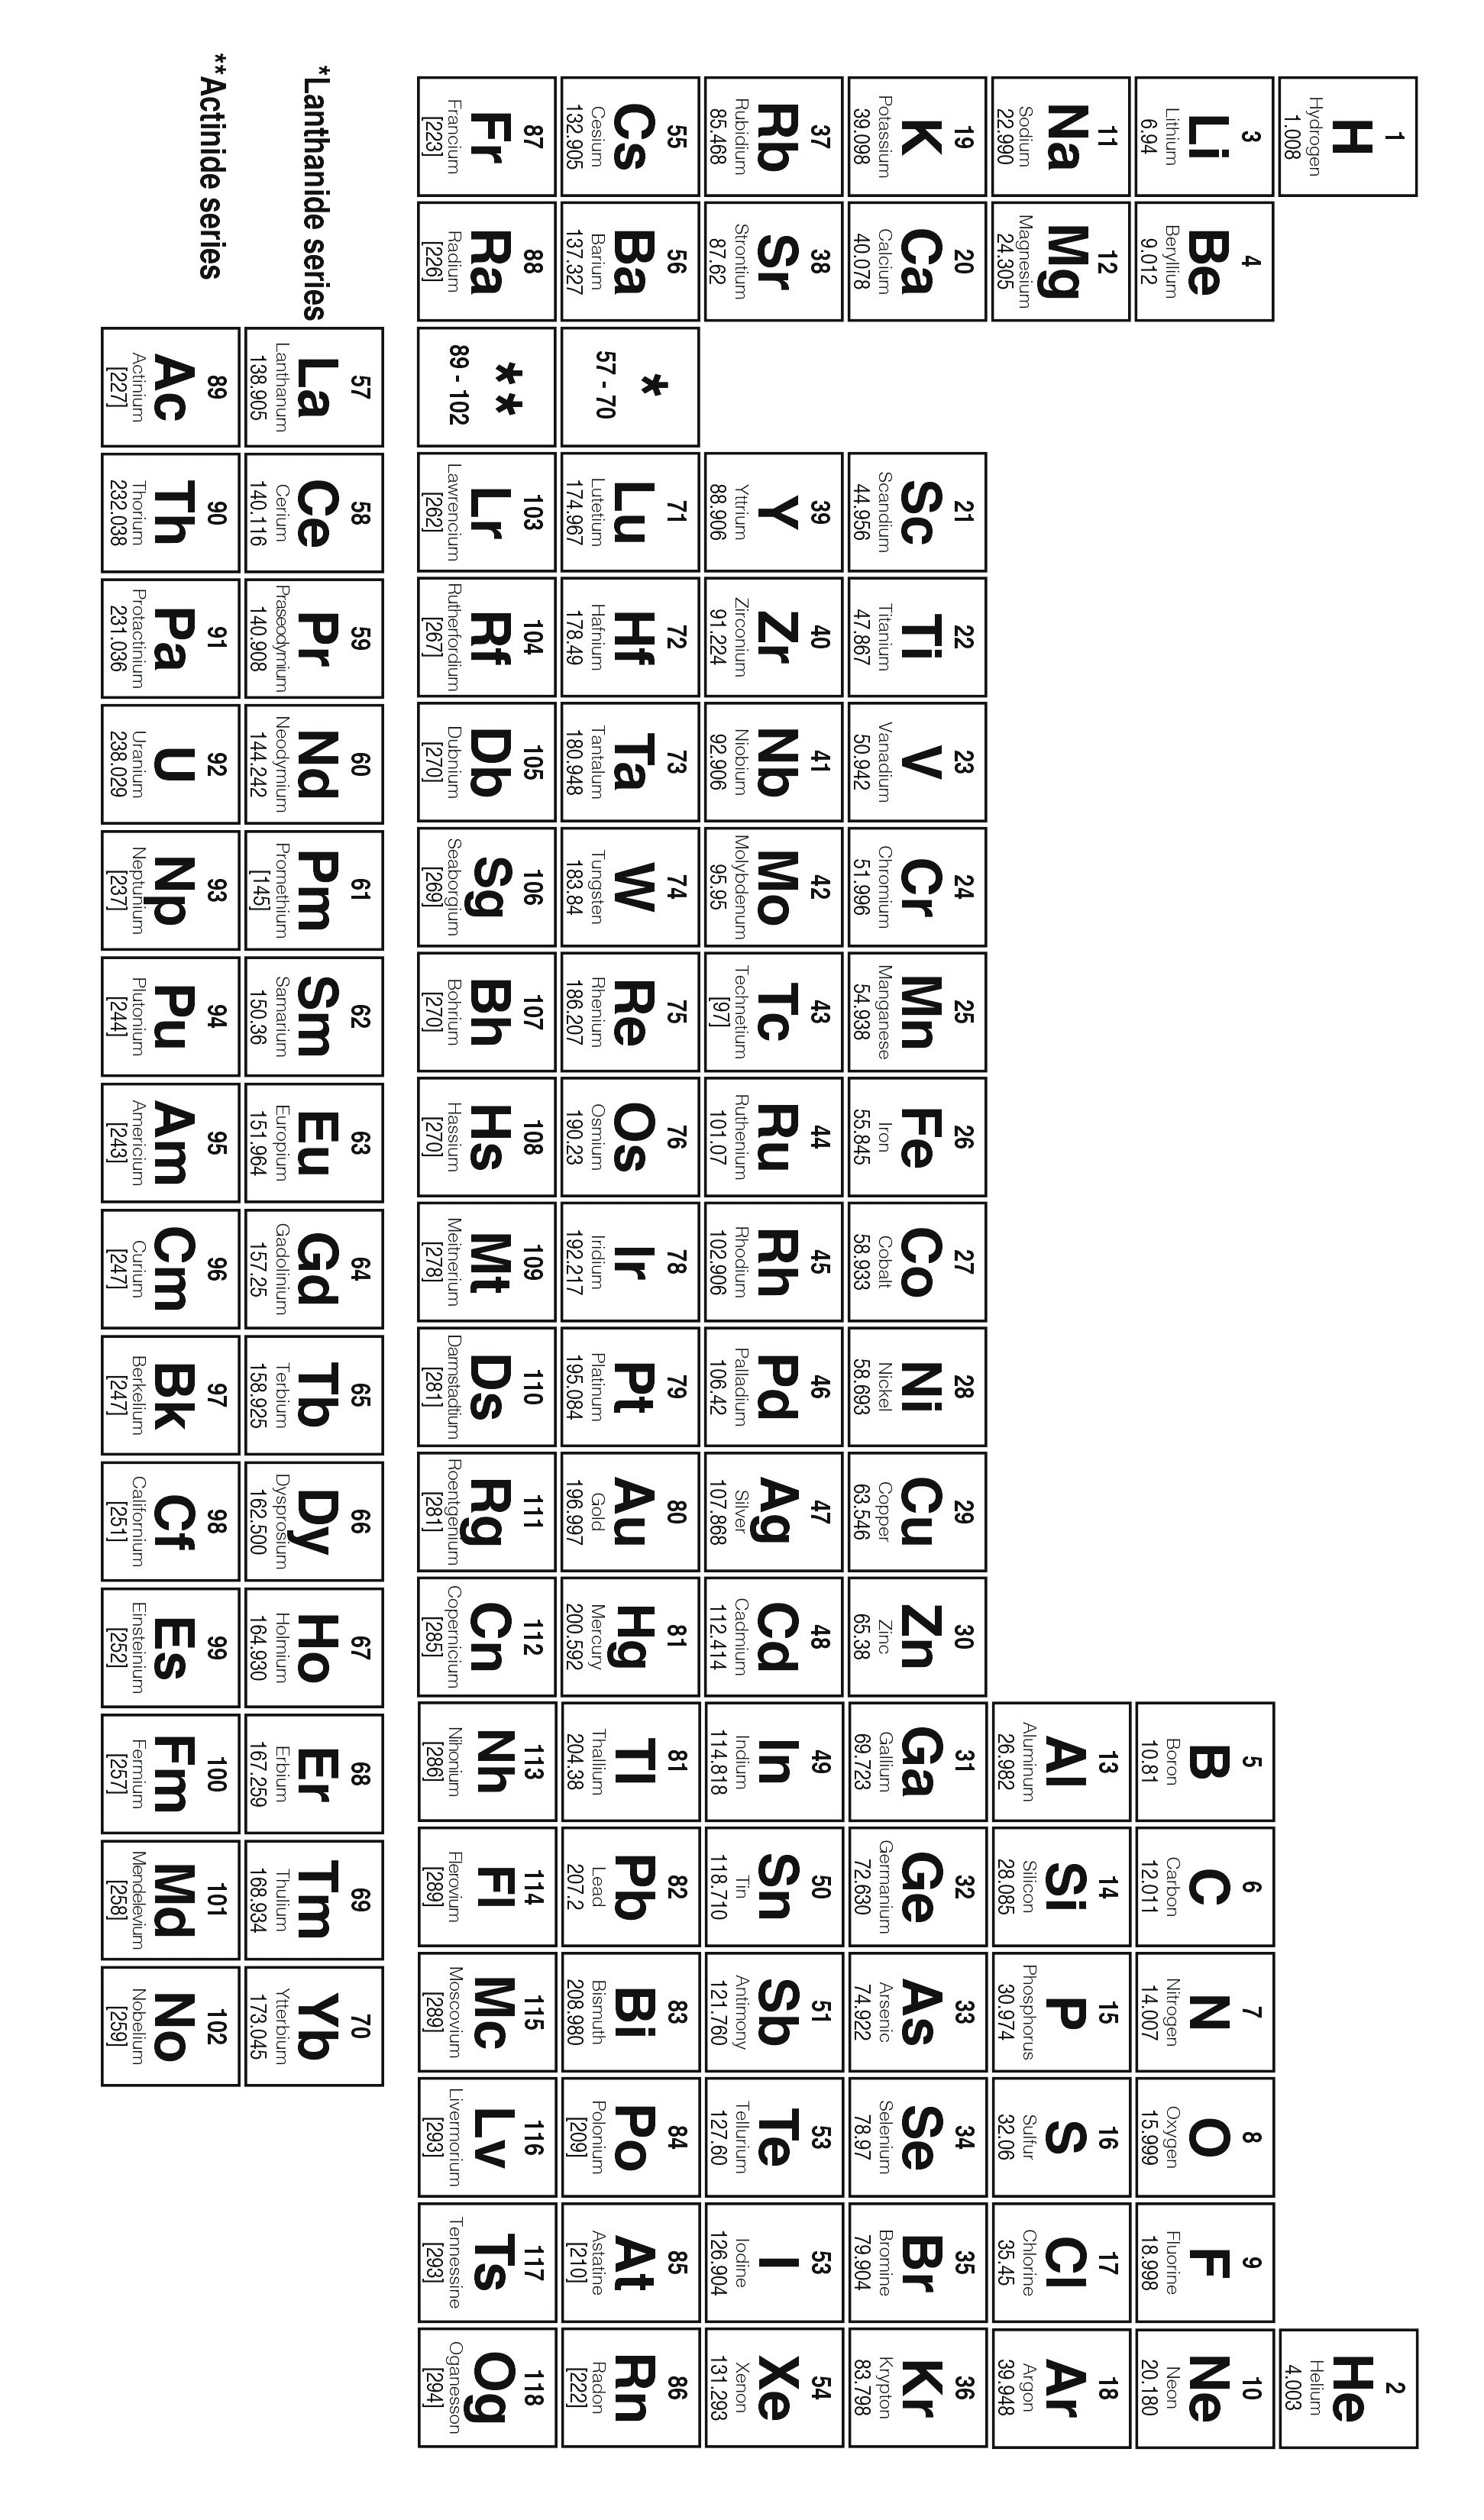
\includegraphics[]{figures/Periodic_Table_Of_Elements_Atomic_Mass_Black_And_White.jpg}
\restoregeometry
\newpage